\section{Embedded Linux development environment}

\begin{frame}
  \frametitle{Embedded Linux solutions}
  \begin{itemize}
  \item Two ways to switch to embedded Linux
    \begin{itemize}
    \item Use {\bf solutions provided and supported by vendors} like
      MontaVista, Wind River or TimeSys. These solutions come with
      their own development tools and environment. They use a mix of
      open-source components and proprietary tools.
    \item Use {\bf community solutions}. They are completely open,
      supported by the community.
    \end{itemize}
  \item In Bootlin training sessions, we do not promote a particular
    vendor, and therefore use community solutions
    \begin{itemize}
    \item However, knowing the concepts, switching to vendor solutions will be easy
    \end{itemize}
  \end{itemize}
\end{frame}

\begin{frame}
  \frametitle{OS for Linux development}
  We strongly recommend to use GNU/Linux as the desktop operating
  system to embedded Linux developers, for multiple reasons.
  \begin{itemize}
  \item All community tools are developed and designed to run on
    Linux. Trying to use them on other operating systems (Windows,
    macOS) will lead to trouble.
  \item As Linux also runs on the embedded device, all the knowledge
    gained from using Linux on the desktop will apply similarly to the
    embedded device.
  \item If you are stuck with a Windows desktop, at least you should
    use GNU/Linux in a virtual machine (such as VirtualBox which is open
    source), though there could be a small performance penalty.
    With Windows 10/11, you can also run your favorite native Linux distro through
    Windows Subsystem for Linux (WSL2)
  \end{itemize}
  \begin{center}
    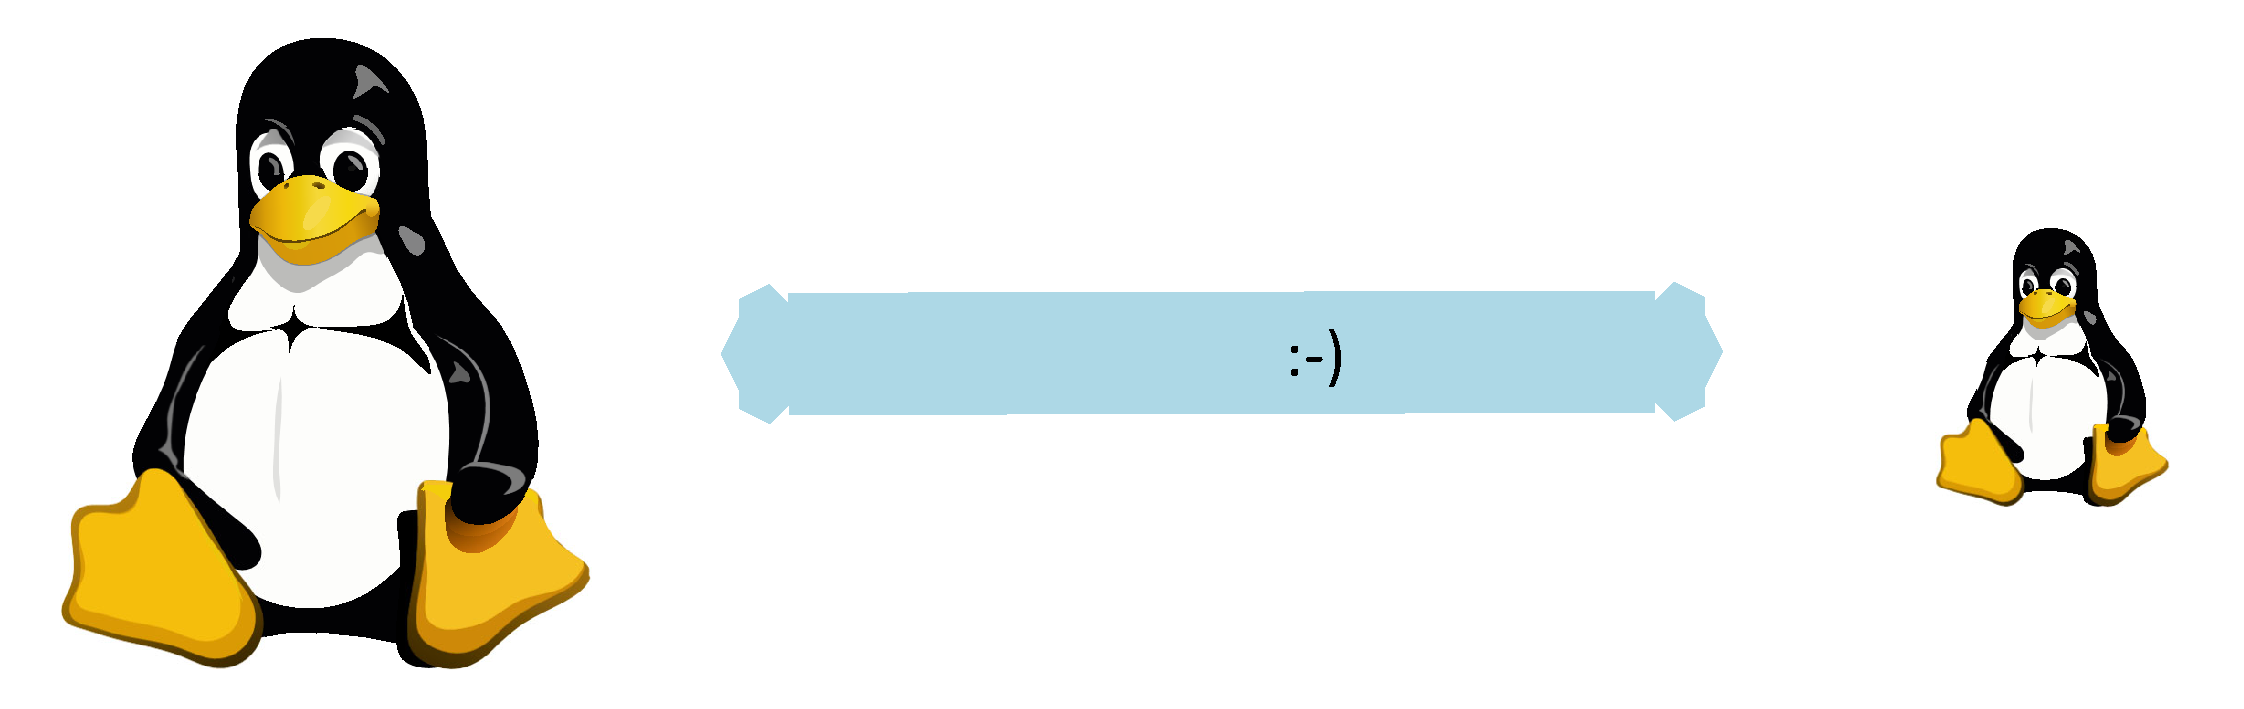
\includegraphics[width=0.5\textwidth]{slides/sysdev-dev-environment/linux-as-development-os.pdf}
  \end{center}
\end{frame}

\begin{frame}
  \frametitle{Desktop Linux distribution}
  \begin{columns}
    \begin{column}{0.7\textwidth}
    \begin{itemize}
    \item {\bf Any good and sufficiently recent Linux desktop
        distribution} can be used for the development workstation
      \begin{itemize}
      \item Ubuntu, Debian, Fedora, openSUSE, Arch Linux, etc.
      \end{itemize}
    \item We have chosen Ubuntu, derived from Debian, as it is a
      {\bf widely used and easy to use} desktop Linux distribution.
    \item The Ubuntu setup on the training laptops has intentionally
      been left untouched after the normal installation
      process. Learning embedded Linux is also about learning the tools
      needed on the development workstation!
    \end{itemize}
    \end{column}
    \begin{column}[t]{0.3\textwidth}
      
\includegraphics[width=0.9\textwidth]{common/ubuntu.pdf}\\
      \tiny Image credits: \url{https://tinyurl.com/f4zxj5kw}
    \end{column}
  \end{columns}
\end{frame}

\begin{frame}
  \frametitle{Host vs. target}
  \begin{itemize}
  \item When doing embedded development, there is always a split between
    \begin{itemize}
    \item The {\em host}, the development workstation, which is
      typically a powerful PC
    \item The {\em target}, which is the embedded system under
      development
    \end{itemize}
  \item They are connected by various means: almost always a serial
    line for debugging purposes, frequently a networking connection,
    sometimes a JTAG interface for low-level debugging
  \end{itemize}
  \begin{center}
    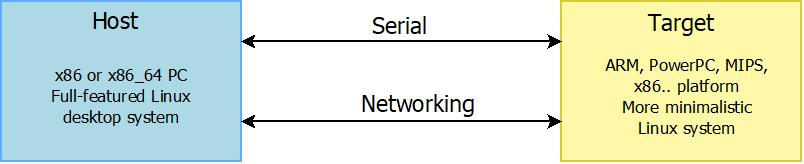
\includegraphics[width=0.7\textwidth]{slides/sysdev-dev-environment/host-vs-target.jpg}
  \end{center}
\end{frame}

\begin{frame}
  \frametitle{Serial line communication program}
  \begin{itemize}
  \item An essential tool for embedded development is a serial line
    communication program, like {\em HyperTerminal} in Windows.
  \item There are multiple options available in Linux: {\em Minicom},
    {\em Picocom}, {\em Gtkterm}, {\em Putty}, {\em screen}, {\em tmux}
    and the new {\em tio} (\url{https://github.com/tio/tio}).
  \item In this training session, we recommend using the simplest of
    them: {\em Picocom}
    \begin{itemize}
    \item Installation with \code{sudo apt install picocom}
    \item Run with \code{picocom -b BAUD_RATE /dev/SERIAL_DEVICE}.
    \item Exit with \code{[Ctrl][a] [Ctrl][x]}
    \end{itemize}
  \item \code{SERIAL_DEVICE} is typically
    \begin{itemize}
    \item \code{ttyUSBx} for USB to serial converters
    \item \code{ttySx} for real serial ports
    \end{itemize}
  \item Most frequent command: \code{picocom -b 115200 /dev/ttyUSB0}
  \end{itemize}
\end{frame}
